\documentclass{standalone}
\usepackage{tikz}
\usetikzlibrary{arrows}

\begin{document}
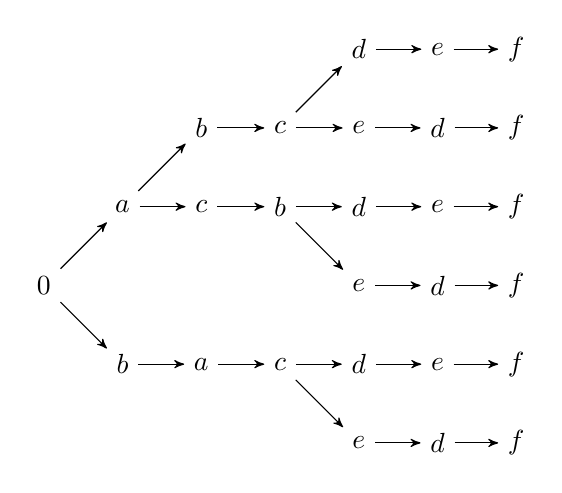
\begin{tikzpicture}[>=stealth']
\node (0) {$0$};
\node (a1) at (1,1) {$a$};
\node (b1) at (1,-1) {$b$};
\node (b2) at (2,2) {$b$};
\node (c2) at (2,1) {$c$};
\node (a2) at (2,-1) {$a$};
\node (c3) at (3,2) {$c$};
\node (b3) at (3,1) {$b$};
\node (c3b) at (3,-1) {$c$};
\node (d43) at (4,3) {$d$};
\node (e43) at (4,2) {$e$};
\node (d42) at (4,1) {$d$};
\node (e42) at (4,0) {$e$};
\node (d41) at (4,-1) {$d$};
\node (e41) at (4,-2) {$e$};
\node (e53) at (5,3) {$e$};
\node (d53) at (5,2) {$d$};
\node (e52) at (5,1) {$e$};
\node (d52) at (5,0) {$d$};
\node (e51) at (5,-1) {$e$};
\node (d51) at (5,-2) {$d$};
\node (f6) at (6,3) {$f$};
\node (f5) at (6,2) {$f$};
\node (f4) at (6,1) {$f$};
\node (f3) at (6,0) {$f$};
\node (f2) at (6,-1) {$f$};
\node (f1) at (6,-2) {$f$};
\draw[->] (0) edge (a1);
\draw[->] (0) edge (b1);
\draw[->] (a1) edge (b2);
\draw[->] (a1) edge (c2);
\draw[->] (b1) edge (a2);
\draw[->] (b2) edge (c3);
\draw[->] (c2) edge (b3);
\draw[->] (a2) edge (c3b);
\draw[->] (c3) edge (d43);
\draw[->] (c3) edge (e43);
\draw[->] (b3) edge (d42);
\draw[->] (b3) edge (e42);
\draw[->] (c3b) edge (d41);
\draw[->] (c3b) edge (e41);
\draw[->] (d43) edge (e53);
\draw[->] (e43) edge (d53);
\draw[->] (d42) edge (e52);
\draw[->] (e42) edge (d52);
\draw[->] (d41) edge (e51);
\draw[->] (e41) edge (d51);
\draw[->] (e53) edge (f6);
\draw[->] (d53) edge (f5);
\draw[->] (e52) edge (f4);
\draw[->] (d52) edge (f3);
\draw[->] (e51) edge (f2);
\draw[->] (d51) edge (f1);
\end{tikzpicture}
\end{document}